\documentclass[letter]{article}
\usepackage{fancyhdr,lastpage,hyperref,soul,graphicx}
\usepackage[T1]{fontenc}
%\usepackage{showframe,lipsum}

\voffset = -0.8in
\hoffset = -0.25in
\oddsidemargin = 0in
\evensidemargin = 0in
\headsep = 0.2in
\headheight = 0.8in
\textheight = 9.5in
\textwidth = 7in

\linespread{1.1}

\pagestyle{fancy}
\lhead{\it Xiaoyu Tai, \href{http://taixiaoyu.com}{\underline{\smash{taixiaoyu.com}}}}
\chead{\LARGE \bfseries\textsc{DMS 423 Final Project - Fall 2014\linebreak}}
\rhead{\it Real-time Satellite Visualization}
\lfoot{}
\cfoot{}
\rfoot{}
%\renewcommand\headrulewidth{0.5pt}

\begin{document}
\begin{flushleft}
\section{About}
This project is designed to be a real-time satellite tracking application. It has a 3D globe with satellites on it. It also has the necessary informations on the top of screen. The view point can be rotated in many ways to archive certain angle.\linebreak
\linebreak
In project B, I create a game called random guess. The application can get any point's coordinates from the globe and turns it into real world address. Therefore, we can guess the address for a certain satellite and check if we have the right guess.
\section{Controls}
\subsection{Project A}
1. Use arrow keys/drag mouse to move the globe\linebreak
2. Use A/W/S/D to rotate the globe in different ways\linebreak
3. Reset the view point by click Q(x-axis rotation), E(z-axis rotation), N(all rotation and back to UB)\linebreak
4. Use Z/X to zoom in and out\linebreak
5. Use G/H to show/hide the satellites's trace lines\linebreak
6. Use number key 1-7 to select satellite sets
\subsection{Project B}
All control methods from \bf Project A\rm, plus:\linebreak
7. Use R to randomly select a satellite on-screen and output the address below it\linebreak
8. Use E to randomly give a point on earth and output its real-world address\linebreak
9. Move the globe and press T for the address of the current point (center of the cross)
\section{Screen Shots}
\begin{center}
    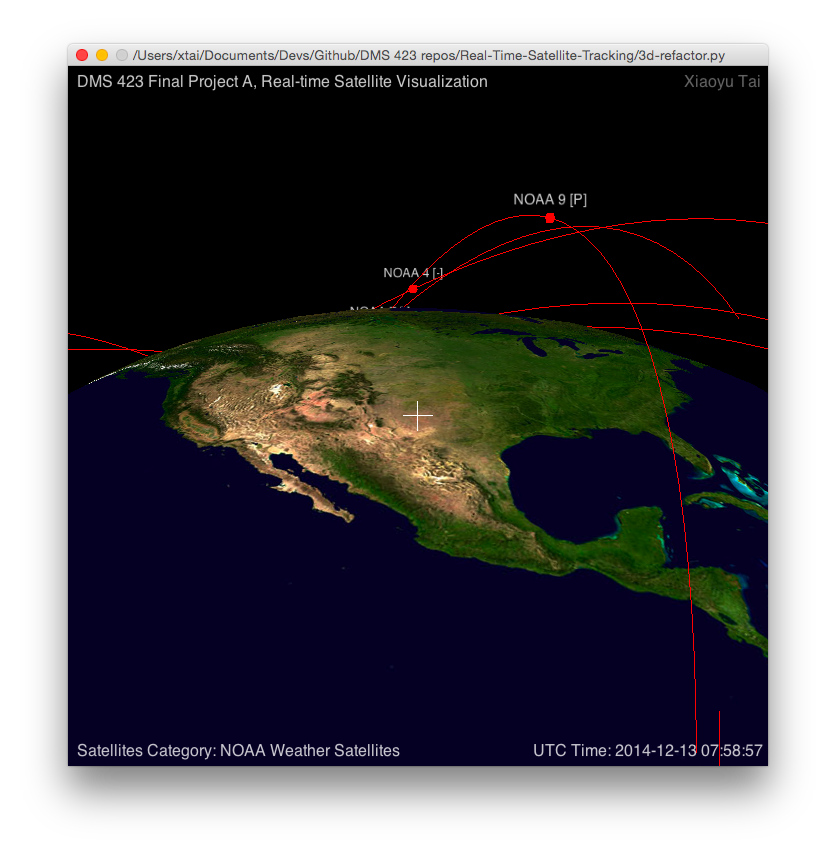
\includegraphics[width=3.5in]{1.png}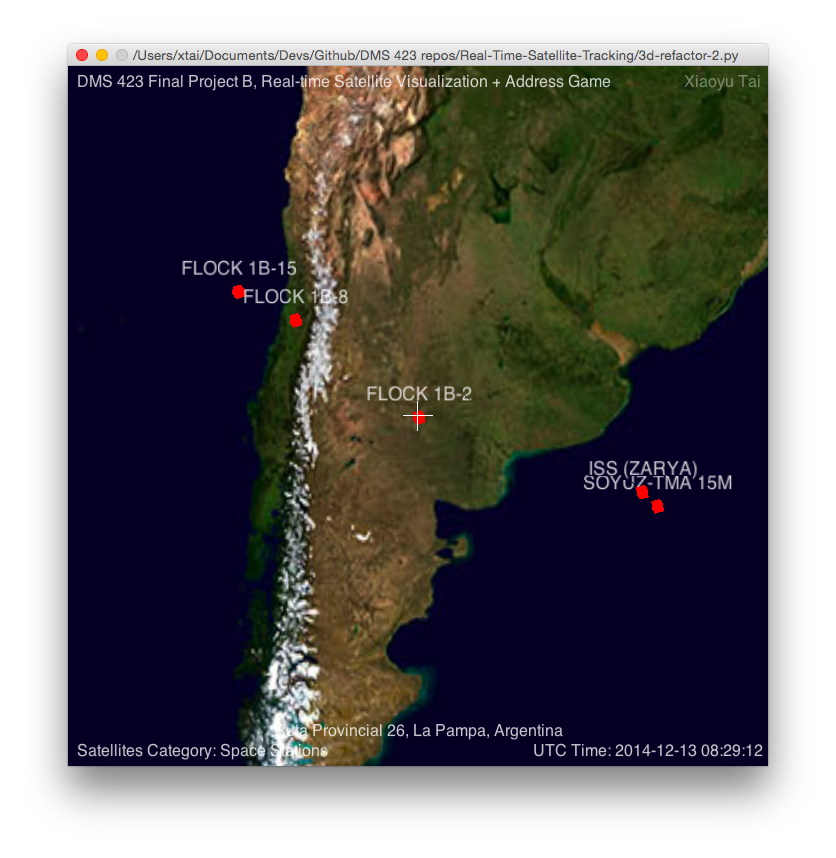
\includegraphics[width=3.5in]{2.png}
    
\end{center}
\end{flushleft}
\end{document}